\documentclass[english,10pt,a4paper,oneside]{book}
\usepackage[english]{babel}

% PAGE GEOMETRY
\usepackage{geometry}
\geometry{margin=4cm}

% FONTS
% with lining figures for math roman; load before other text specs:
% \usepackage{eulervm}
\usepackage{amssymb,amsmath}
\usepackage{ifxetex}
\ifxetex
  \usepackage{microtype}
  \usepackage{mathspec} % only with xelatex; before fontspec
  \usepackage{fontspec} % only with xelatex
  % \defaultfontfeatures{Ligatures=Common}
  \setmainfont[Ligatures=TeX]{Minion Pro}
  \setsansfont[Ligatures=TeX,Scale=MatchLowercase]{Myriad Pro}
  \setmonofont[Scale=.85]{Ubuntu Mono}
  % custom ampersand
  \newcommand{\amper}{{\fontspec[Scale=.95]{Hoefler Text}\selectfont\itshape\&}}
\else
  \usepackage[activate={true,nocompatibility},final,tracking=true,kerning=true,spacing=true,factor=1100,stretch=10,shrink=10]{microtype}
  \usepackage[T1]{fontenc}
  \usepackage[utf8]{inputenc}
  \DeclareUnicodeCharacter{2212}{-}
\fi

% TYPOGRAPHY SETTINGS
% disable protrusion for tt fonts
\UseMicrotypeSet[protrusion]{basicmath}
% remove excessive space after full-stop
\frenchspacing

% % CHAPTER HEADINGS
% \usepackage{sectsty} % don't work with 'quotchap'
% \chapterfont{\usefont{T1}{qhv}{b}{n}\selectfont\huge}
% qotation ahead of chapters and fancy chapter heading
\usepackage{quotchap}
\renewcommand*{\sectfont}{\sffamily\bfseries\Huge\selectfont}

% SECTION, SUBSECTION, ETC. TITLES
\usepackage[compact]{titlesec}
% \titleformat{\chapter} % don't work with 'quotchap'
%   {\normalfont\Huge\sffamily\bfseries}
%   {\thechapter}
%   {1em}
%   {}
\titleformat{\section}
  {\normalfont\LARGE\sffamily\bfseries}
  {\thesection}
  {1em}
  {}
\titleformat{\subsection}
  {\normalfont\Large\sffamily\bfseries}
  {\thesubsection}
  {1em}
  {}
\titleformat{\subsubsection}
  {\normalfont\large\sffamily\bfseries\slshape}
  {\thesubsubsection}
  {1em}
  {}
% \titlespacing*{<command>}{<left>}{<before-sep>}{<after-sep>}
\titlespacing*{\section}
  {0pt}
  {1.2ex plus 1ex minus .2ex}
  {0.5ex plus .1ex minus .1ex}
\titlespacing*{\subsection}
  {0pt}
  {1.2ex plus 1ex minus .2ex}
  {0.5ex plus .1ex minus .1ex}
\titlespacing*{\subsubsection}
  {0pt}
  {1.2ex plus 1ex minus .2ex}
  {0.5ex plus .1ex minus .1ex}

% FIGURE AND TABLE CAPTIONS
\usepackage{floatrow}
\floatsetup[figure]{capposition=bottom}
\floatsetup[table]{capposition=top}

% QUOTATIONS AND QUOTATION MARKS
\usepackage[autostyle]{csquotes} % works with babel
% use upquote if available, for straight quotes in verbatim environments
\usepackage{upquote}{}

% HYPERLINKS
\usepackage{hyperref}
\hypersetup{
    colorlinks=true,
    linkcolor=blue,
    filecolor=magenta,
    urlcolor=cyan,
}
\urlstyle{same}
% avoid problems with \sout in headers with hyperref
\usepackage[normalem]{ulem}
\pdfstringdefDisableCommands{\renewcommand{\sout}{}}

% FOOTNOTES
\usepackage{fancyvrb}
\VerbatimFootnotes % allows verbatim text in footnotes
% Make links footnotes instead of hotlinks
\renewcommand{\href}[2]{#2\footnote{\url{#1}}}
% Use protect on footnotes to avoid problems with footnotes in titles
\let\rmarkdownfootnote\footnote%
\def\footnote{\protect\rmarkdownfootnote}

% BIBLIOGRAPHY
\usepackage{natbib}

% TABLES
\usepackage{longtable,booktabs,tabularx,ragged2e,dcolumn,multirow,multicol}
\setlength\heavyrulewidth{0.1em}
\setlength\lightrulewidth{0.0625em}

% SI UNITS
\usepackage{siunitx}
    \sisetup{%
        detect-mode,
        group-digits            = false,
        input-symbols           = ( ) [ ] - + < > * §,
        table-align-text-post   = false,
        round-mode              = places,
        round-precision         = 3
        }

% GRAPHICS SETTINGS
\usepackage{graphicx,grffile}
\makeatletter
\def\maxwidth{\ifdim\Gin@nat@width>\linewidth\linewidth\else\Gin@nat@width\fi}
\def\maxheight{\ifdim\Gin@nat@height>\textheight\textheight\else\Gin@nat@height\fi}
\makeatother
% Scale images if necessary, so that they will not overflow the page
% margins by default, and it is still possible to overwrite the defaults
% using explicit options in \includegraphics[width, height, ...]{}
\setkeys{Gin}{width=\maxwidth,height=\maxheight,keepaspectratio}

% LINESPACING
% \usepackage{setspace}
% \setstretch{1.5}

% NO INDENTATION WITH A SPACE BETWEEN PARAGRAPHS
\usepackage{parskip}
\setlength{\parindent}{0pt}
\setlength{\parskip}{6pt plus 2pt minus 1pt}
% prevent overfull lines
\setlength{\emergencystretch}{3em}
\providecommand{\tightlist}{%
  \setlength{\itemsep}{0pt}\setlength{\parskip}{0pt}}

% THE NEXT LINES OF CODE SPECIFY SOME YAML ENTRIES %
%%%%%%%%%%%%%%%%%%%%%%%%%%%%%%%%%%%%%%%%%%%%%%%%%%%%
% switch yes/no in YAML header

% ENABLES LISTING OF CODE (echo = TRUE)
% listings: yes/no
\usepackage{color}
\usepackage{fancyvrb}
\newcommand{\VerbBar}{|}
\newcommand{\VERB}{\Verb[commandchars=\\\{\}]}
\DefineVerbatimEnvironment{Highlighting}{Verbatim}{commandchars=\\\{\}}
% Add ',fontsize=\small' for more characters per line
\usepackage{framed}
\definecolor{shadecolor}{RGB}{248,248,248}
\newenvironment{Shaded}{\begin{snugshade}}{\end{snugshade}}
\newcommand{\AlertTok}[1]{\textcolor[rgb]{0.94,0.16,0.16}{#1}}
\newcommand{\AnnotationTok}[1]{\textcolor[rgb]{0.56,0.35,0.01}{\textbf{\textit{#1}}}}
\newcommand{\AttributeTok}[1]{\textcolor[rgb]{0.77,0.63,0.00}{#1}}
\newcommand{\BaseNTok}[1]{\textcolor[rgb]{0.00,0.00,0.81}{#1}}
\newcommand{\BuiltInTok}[1]{#1}
\newcommand{\CharTok}[1]{\textcolor[rgb]{0.31,0.60,0.02}{#1}}
\newcommand{\CommentTok}[1]{\textcolor[rgb]{0.56,0.35,0.01}{\textit{#1}}}
\newcommand{\CommentVarTok}[1]{\textcolor[rgb]{0.56,0.35,0.01}{\textbf{\textit{#1}}}}
\newcommand{\ConstantTok}[1]{\textcolor[rgb]{0.00,0.00,0.00}{#1}}
\newcommand{\ControlFlowTok}[1]{\textcolor[rgb]{0.13,0.29,0.53}{\textbf{#1}}}
\newcommand{\DataTypeTok}[1]{\textcolor[rgb]{0.13,0.29,0.53}{#1}}
\newcommand{\DecValTok}[1]{\textcolor[rgb]{0.00,0.00,0.81}{#1}}
\newcommand{\DocumentationTok}[1]{\textcolor[rgb]{0.56,0.35,0.01}{\textbf{\textit{#1}}}}
\newcommand{\ErrorTok}[1]{\textcolor[rgb]{0.64,0.00,0.00}{\textbf{#1}}}
\newcommand{\ExtensionTok}[1]{#1}
\newcommand{\FloatTok}[1]{\textcolor[rgb]{0.00,0.00,0.81}{#1}}
\newcommand{\FunctionTok}[1]{\textcolor[rgb]{0.00,0.00,0.00}{#1}}
\newcommand{\ImportTok}[1]{#1}
\newcommand{\InformationTok}[1]{\textcolor[rgb]{0.56,0.35,0.01}{\textbf{\textit{#1}}}}
\newcommand{\KeywordTok}[1]{\textcolor[rgb]{0.13,0.29,0.53}{\textbf{#1}}}
\newcommand{\NormalTok}[1]{#1}
\newcommand{\OperatorTok}[1]{\textcolor[rgb]{0.81,0.36,0.00}{\textbf{#1}}}
\newcommand{\OtherTok}[1]{\textcolor[rgb]{0.56,0.35,0.01}{#1}}
\newcommand{\PreprocessorTok}[1]{\textcolor[rgb]{0.56,0.35,0.01}{\textit{#1}}}
\newcommand{\RegionMarkerTok}[1]{#1}
\newcommand{\SpecialCharTok}[1]{\textcolor[rgb]{0.00,0.00,0.00}{#1}}
\newcommand{\SpecialStringTok}[1]{\textcolor[rgb]{0.31,0.60,0.02}{#1}}
\newcommand{\StringTok}[1]{\textcolor[rgb]{0.31,0.60,0.02}{#1}}
\newcommand{\VariableTok}[1]{\textcolor[rgb]{0.00,0.00,0.00}{#1}}
\newcommand{\VerbatimStringTok}[1]{\textcolor[rgb]{0.31,0.60,0.02}{#1}}
\newcommand{\WarningTok}[1]{\textcolor[rgb]{0.56,0.35,0.01}{\textbf{\textit{#1}}}}

% NUMBERED SECTIONS OR NOT
% numbersections: yes/no
\setcounter{secnumdepth}{5}

% REDEFINE SUBPARAGRAPHS
% subparagraph: yes
% Redefines (sub)paragraphs to behave more like sections
\ifx\paragraph\undefined\else
\let\oldparagraph\paragraph
\renewcommand{\paragraph}[1]{\oldparagraph{#1}\mbox{}}
\fi
\ifx\subparagraph\undefined\else
\let\oldsubparagraph\subparagraph
\renewcommand{\subparagraph}[1]{\oldsubparagraph{#1}\mbox{}}
\fi

% COMPACT TITLES
% CREATE SUBTITLE COMMAND FOR USE IN MAKETITLE
\usepackage{titling}
\newcommand{\subtitle}[1]{
  \posttitle{
    \begin{center}\large#1\end{center}
    }
}

% YAML ENTRIES: 'title', 'subtitle', 'author' and 'date'
\setlength{\droptitle}{-2em}
  \title{Basic Statistics}
  \pretitle{\vspace{\droptitle}\centering\huge}
  \posttitle{\par}
\subtitle{\sf A primer in basic statistics for BCB (Hons) 2019}
  \author{AJ Smit and Robert Schlegel}
  \preauthor{\centering\large\emph}
  \postauthor{\par}
  \predate{\centering\large\emph}
  \postdate{\par}
  \date{2019-04-09}

% COMMENT IF FIGURE ABOVE TITLE IS NOT REQUIRED
% \pretitle{%
%   \begin{center}
%   \LARGE
%   
\includegraphics[width=5cm]{figures/769_life_finds_a_way.png}\\[\bigskipamount]
% }
% \posttitle{\end{center}}

% ANY HEADER/PREAMBLE LaTeX code can be added to the file
% specified here by
% header-includes: path/to/the/file.tex

\begin{document}
\maketitle



% TABLE OF CONTENT
% toc: yes/no
{
\hypersetup{linkcolor=black}
\setcounter{tocdepth}{2}
\tableofcontents
}

% LIST OF TABLES
\listoftables

% LIST OF FIGURES
\listoffigures

\hypertarget{preface}{%
\chapter*{Preface}\label{preface}}


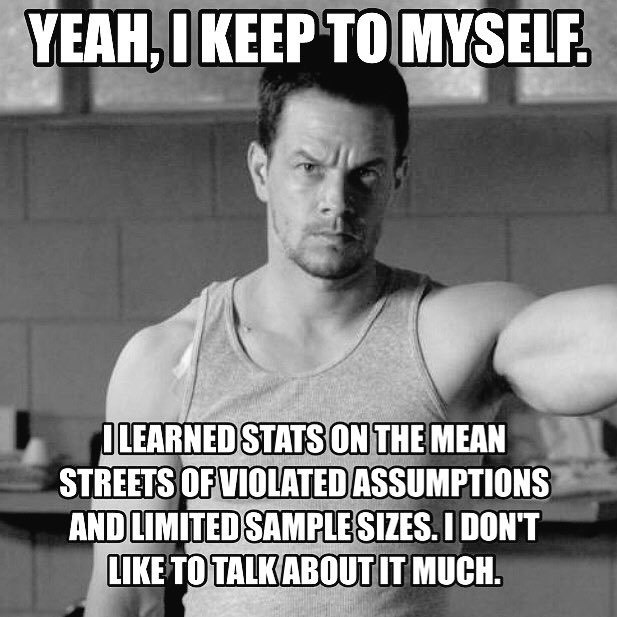
\includegraphics[width=0.7\linewidth]{figures/walberg_assumptions}

This is a workshop about the practice of the basic statistics used by biologists, and not about the theory and mathematical underpinnings of the methods used. Each of the Chapters will cover a basic kind of statistical approach, and the main classes of data it applies to. Since much insight and understanding can be gained from visualising our data, we will also explore the main types of graphical summaries that best accompany the statistical methodologies. It is our intention to demonstrate how we go about analysing our data.

\hypertarget{prerequisites}{%
\chapter*{Prerequisites}\label{prerequisites}}


A prerequisite for this course is a basic proficiency in using R \citep{R2017}. The necessary experience will have been gained from completing the \href{https://robwschlegel.github.io/Intro_R_Workshop/}{Intro R Workshop: Data Manipulation, Analysis, and Graphing} Workshop that was part of your BCB Core Honours module (i.e.~Biostatistics). You will also need a laptop with R and RStudio installed as per the instructions provided in that workshop. If you do not have a personal laptop, most computers in the 5th floor lab will be correctly set up for this purpose.

\hypertarget{introduction}{%
\chapter{Introduction}\label{introduction}}

Placeholder

\hypertarget{venue-date-and-time}{%
\section{Venue, date and time}\label{venue-date-and-time}}

\hypertarget{course-outline}{%
\section{Course outline}\label{course-outline}}

\hypertarget{about-this-workshop}{%
\section{About this Workshop}\label{about-this-workshop}}

\hypertarget{this-is-biology-why-more-r-coding}{%
\section{This is biology: why more R coding?}\label{this-is-biology-why-more-r-coding}}

\hypertarget{installing-r-and-rstudio}{%
\section{Installing R and RStudio}\label{installing-r-and-rstudio}}

\hypertarget{resources}{%
\section{Resources}\label{resources}}

\hypertarget{style-and-code-conventions}{%
\section{Style and code conventions}\label{style-and-code-conventions}}

\hypertarget{assessment-and-teaching-philosophy}{%
\section{Assessment and teaching philosophy}\label{assessment-and-teaching-philosophy}}

\hypertarget{about-this-document}{%
\section{About this document}\label{about-this-document}}

\hypertarget{types-of-data}{%
\chapter{Types of data}\label{types-of-data}}

Placeholder

\hypertarget{data-classes}{%
\section{Data classes}\label{data-classes}}

\hypertarget{numerical-data}{%
\subsection{Numerical data}\label{numerical-data}}

\hypertarget{nominal-discrete-data}{%
\subsubsection{Nominal (discrete) data}\label{nominal-discrete-data}}

\hypertarget{continuous-data}{%
\subsubsection{Continuous data}\label{continuous-data}}

\hypertarget{dates}{%
\subsubsection{Dates}\label{dates}}

\hypertarget{qualitative-data}{%
\subsection{Qualitative data}\label{qualitative-data}}

\hypertarget{categorical-data}{%
\subsubsection{Categorical data}\label{categorical-data}}

\hypertarget{ordinal-data}{%
\subsubsection{Ordinal data}\label{ordinal-data}}

\hypertarget{binary-data}{%
\subsection{Binary data}\label{binary-data}}

\hypertarget{character-values}{%
\subsection{Character values}\label{character-values}}

\hypertarget{missing-values}{%
\subsection{Missing values}\label{missing-values}}

\hypertarget{complex-numbers}{%
\subsection{Complex numbers}\label{complex-numbers}}

\hypertarget{viewing-our-data}{%
\section{Viewing our data}\label{viewing-our-data}}

\hypertarget{from-the-environment-pane}{%
\subsection{From the Environment pane}\label{from-the-environment-pane}}

\hypertarget{head-and-tail}{%
\subsection{\texorpdfstring{\texttt{head()} and \texttt{tail()}}{head() and tail()}}\label{head-and-tail}}

\hypertarget{colnames}{%
\subsection{\texorpdfstring{\texttt{colnames()}}{colnames()}}\label{colnames}}

\hypertarget{summary}{%
\subsection{\texorpdfstring{\texttt{summary()}}{summary()}}\label{summary}}

\hypertarget{descriptive-statistics-central-tendency-and-dispersion}{%
\chapter{Descriptive statistics: central tendency and dispersion}\label{descriptive-statistics-central-tendency-and-dispersion}}

Placeholder

\hypertarget{samples-and-populations}{%
\section{Samples and populations}\label{samples-and-populations}}

\hypertarget{measures-of-central-tendency}{%
\section{Measures of central tendency}\label{measures-of-central-tendency}}

\hypertarget{the-mean}{%
\subsection{The mean}\label{the-mean}}

\hypertarget{the-median}{%
\subsection{The median}\label{the-median}}

\hypertarget{skewness}{%
\subsection{Skewness}\label{skewness}}

\hypertarget{kurtosis}{%
\subsection{Kurtosis}\label{kurtosis}}

\hypertarget{measures-of-variation-and-spread}{%
\section{Measures of variation and spread}\label{measures-of-variation-and-spread}}

\hypertarget{the-variance-and-standard-deviation}{%
\subsection{The variance and standard deviation}\label{the-variance-and-standard-deviation}}

\hypertarget{quantiles}{%
\subsection{Quantiles}\label{quantiles}}

\hypertarget{the-minimum-maximum-and-range}{%
\subsection{The minimum, maximum and range}\label{the-minimum-maximum-and-range}}

\hypertarget{covariance}{%
\subsection{Covariance}\label{covariance}}

\hypertarget{correlation}{%
\subsection{Correlation}\label{correlation}}

\hypertarget{missing-values-1}{%
\section{Missing values}\label{missing-values-1}}

\hypertarget{descriptive-statistics-by-group}{%
\section{Descriptive statistics by group}\label{descriptive-statistics-by-group}}

\hypertarget{groupwise-summary-statistics}{%
\subsection{Groupwise summary statistics}\label{groupwise-summary-statistics}}

\hypertarget{displays-of-group-summaries}{%
\subsection{Displays of group summaries}\label{displays-of-group-summaries}}

\hypertarget{exercises}{%
\section{Exercises}\label{exercises}}

\hypertarget{exercise-1}{%
\subsection{Exercise 1}\label{exercise-1}}

\hypertarget{graphical-data-displays}{%
\chapter{Graphical data displays}\label{graphical-data-displays}}

Placeholder

\hypertarget{qualitative-data-1}{%
\section{Qualitative data}\label{qualitative-data-1}}

\hypertarget{continuous-data-1}{%
\section{Continuous data}\label{continuous-data-1}}

\hypertarget{frequency-distributions-histograms}{%
\subsection{Frequency distributions (histograms)}\label{frequency-distributions-histograms}}

\hypertarget{box-plots}{%
\subsection{Box plots}\label{box-plots}}

\hypertarget{pairwise-scatter-plots}{%
\subsection{Pairwise Scatter plots}\label{pairwise-scatter-plots}}

\hypertarget{bar-graphs}{%
\subsection{Bar graphs}\label{bar-graphs}}

\hypertarget{density-graphs}{%
\subsection{Density graphs}\label{density-graphs}}

\hypertarget{violin-plots}{%
\subsection{Violin plots}\label{violin-plots}}

\hypertarget{exercises-1}{%
\section{Exercises}\label{exercises-1}}

\hypertarget{exercise-1-1}{%
\subsection{Exercise 1}\label{exercise-1-1}}

\hypertarget{distributions}{%
\chapter{Distributions}\label{distributions}}

Placeholder

\hypertarget{discrete-distributions}{%
\section{Discrete distributions}\label{discrete-distributions}}

\hypertarget{bernoulli-distribution}{%
\subsection{Bernoulli distribution}\label{bernoulli-distribution}}

\hypertarget{binomial-distribution}{%
\subsection{Binomial distribution}\label{binomial-distribution}}

\hypertarget{negative-binomial-distribution}{%
\subsection{Negative binomial distribution}\label{negative-binomial-distribution}}

\hypertarget{geometric-distribution}{%
\subsection{Geometric distribution}\label{geometric-distribution}}

\hypertarget{poisson-distribution}{%
\subsection{Poisson distribution}\label{poisson-distribution}}

\hypertarget{continuous-distributions}{%
\section{Continuous distributions}\label{continuous-distributions}}

\hypertarget{normal-distribution}{%
\subsection{Normal distribution}\label{normal-distribution}}

\hypertarget{uniform-distribution}{%
\subsection{Uniform distribution}\label{uniform-distribution}}

\hypertarget{student-t-distribution}{%
\subsection{Student T distribution}\label{student-t-distribution}}

\hypertarget{chi-squared-distribution}{%
\subsection{Chi-squared distribution}\label{chi-squared-distribution}}

\hypertarget{exponential-distribution}{%
\subsection{Exponential distribution}\label{exponential-distribution}}

\hypertarget{f-distribution}{%
\subsection{F distribution}\label{f-distribution}}

\hypertarget{gamma-distribution}{%
\subsection{Gamma distribution}\label{gamma-distribution}}

\hypertarget{beta-distribution}{%
\subsection{Beta distribution}\label{beta-distribution}}

\hypertarget{paranormal-distributions}{%
\subsection{Paranormal distributions}\label{paranormal-distributions}}

\hypertarget{finding-ones-data-distribution}{%
\section{Finding one's data distribution}\label{finding-ones-data-distribution}}

\hypertarget{exercises-2}{%
\section{Exercises}\label{exercises-2}}

\hypertarget{exercise-1-2}{%
\subsection{Exercise 1}\label{exercise-1-2}}

\hypertarget{inferences-about-one-or-two-populations}{%
\chapter{Inferences about one or two populations}\label{inferences-about-one-or-two-populations}}

Placeholder

\hypertarget{assumptions}{%
\section{Assumptions}\label{assumptions}}

\hypertarget{normality}{%
\subsection{Normality}\label{normality}}

\hypertarget{homoscedasticity}{%
\subsection{Homoscedasticity}\label{homoscedasticity}}

\hypertarget{two-for-one}{%
\subsection{Two for one}\label{two-for-one}}

\hypertarget{one-sample-t-tests}{%
\section{\texorpdfstring{One-sample \emph{t}-tests}{One-sample t-tests}}\label{one-sample-t-tests}}

\hypertarget{one-sided-one-sample-t-tests}{%
\subsection{\texorpdfstring{One-sided one-sample \emph{t}-tests}{One-sided one-sample t-tests}}\label{one-sided-one-sample-t-tests}}

\hypertarget{two-sided-one-sample-t-tests}{%
\subsection{\texorpdfstring{Two-sided one-sample \emph{t}-tests}{Two-sided one-sample t-tests}}\label{two-sided-one-sample-t-tests}}

\hypertarget{two-sample-t-tests}{%
\section{\texorpdfstring{Two-sample \emph{t}-tests}{Two-sample t-tests}}\label{two-sample-t-tests}}

\hypertarget{one-sided-two-sample-t-tests}{%
\subsection{\texorpdfstring{One-sided two-sample \emph{t}-tests}{One-sided two-sample t-tests}}\label{one-sided-two-sample-t-tests}}

\hypertarget{two-sided-two-sample-t-tests}{%
\subsection{\texorpdfstring{Two-sided two-sample \emph{t}-tests}{Two-sided two-sample t-tests}}\label{two-sided-two-sample-t-tests}}

\hypertarget{paired-t-tests}{%
\section{\texorpdfstring{Paired \emph{t}-tests}{Paired t-tests}}\label{paired-t-tests}}

\hypertarget{comparison-of-two-population-proportions}{%
\section{Comparison of two population proportions}\label{comparison-of-two-population-proportions}}

\hypertarget{one-sample-and-two-sample-tests}{%
\subsection{One-sample and two-sample tests}\label{one-sample-and-two-sample-tests}}

\hypertarget{one-sided-and-two-sided-tests}{%
\subsection{One-sided and two-sided tests}\label{one-sided-and-two-sided-tests}}

\hypertarget{a-t-test-workflow}{%
\section{\texorpdfstring{A \emph{t}-test workflow}{A t-test workflow}}\label{a-t-test-workflow}}

\hypertarget{loading-data}{%
\subsection{Loading data}\label{loading-data}}

\hypertarget{visualising-data}{%
\subsection{Visualising data}\label{visualising-data}}

\hypertarget{formulating-a-hypothesis}{%
\subsection{Formulating a hypothesis}\label{formulating-a-hypothesis}}

\hypertarget{choosing-a-test}{%
\subsection{Choosing a test}\label{choosing-a-test}}

\hypertarget{checking-assumptions}{%
\subsection{Checking assumptions}\label{checking-assumptions}}

\hypertarget{running-an-analysis}{%
\subsection{Running an analysis}\label{running-an-analysis}}

\hypertarget{interpreting-the-results}{%
\subsection{Interpreting the results}\label{interpreting-the-results}}

\hypertarget{drawing-conclusions}{%
\subsection{Drawing conclusions}\label{drawing-conclusions}}

\hypertarget{going-further}{%
\subsection{Going further}\label{going-further}}

\hypertarget{exercises-3}{%
\section{Exercises}\label{exercises-3}}

\hypertarget{exercise-1-3}{%
\subsection{Exercise 1}\label{exercise-1-3}}

\hypertarget{exercise-2}{%
\subsection{Exercise 2}\label{exercise-2}}

\hypertarget{anova}{%
\chapter{ANOVA}\label{anova}}

Placeholder

\hypertarget{remember-the-t-test}{%
\section{\texorpdfstring{Remember the \emph{t}-test}{Remember the t-test}}\label{remember-the-t-test}}

\hypertarget{anova-1}{%
\section{ANOVA}\label{anova-1}}

\hypertarget{single-factor}{%
\subsection{Single factor}\label{single-factor}}

\hypertarget{multiple-factors}{%
\subsection{Multiple factors}\label{multiple-factors}}

\hypertarget{about-interaction-terms}{%
\subsubsection{About interaction terms}\label{about-interaction-terms}}

\hypertarget{examples}{%
\subsection{Examples}\label{examples}}

\hypertarget{snakes}{%
\subsubsection{Snakes!}\label{snakes}}

\hypertarget{alternatives-to-anova}{%
\section{Alternatives to ANOVA}\label{alternatives-to-anova}}

\hypertarget{wilcox-rank-sum-test}{%
\subsection{Wilcox rank sum test}\label{wilcox-rank-sum-test}}

\hypertarget{kruskall-wallis-rank-sum-test}{%
\subsection{Kruskall-Wallis rank sum test}\label{kruskall-wallis-rank-sum-test}}

\hypertarget{single-factor-1}{%
\subsubsection{Single factor}\label{single-factor-1}}

\hypertarget{multiple-factors-1}{%
\subsubsection{Multiple factors}\label{multiple-factors-1}}

\hypertarget{the-sa-time-data}{%
\subsection{The SA time data}\label{the-sa-time-data}}

\hypertarget{exercises-4}{%
\section{Exercises}\label{exercises-4}}

\hypertarget{exercise-1-4}{%
\subsection{Exercise 1}\label{exercise-1-4}}

\hypertarget{exercise-2-1}{%
\subsection{Exercise 2}\label{exercise-2-1}}

\hypertarget{exercise-3}{%
\subsection{Exercise 3}\label{exercise-3}}

\hypertarget{simple-linear-regressions}{%
\chapter{Simple linear regressions}\label{simple-linear-regressions}}

Placeholder

\hypertarget{the-simple-linear-regression-equation}{%
\section{The simple linear regression equation}\label{the-simple-linear-regression-equation}}

\hypertarget{the-intercept}{%
\subsection{The intercept}\label{the-intercept}}

\hypertarget{the-regression-coefficient}{%
\subsection{The regression coefficient}\label{the-regression-coefficient}}

\hypertarget{a-graph-of-the-linear-regression}{%
\subsection{A graph of the linear regression}\label{a-graph-of-the-linear-regression}}

\hypertarget{predicting-from-the-linear-model}{%
\subsection{Predicting from the linear model}\label{predicting-from-the-linear-model}}

\hypertarget{the-coefficient-of-determination-r2}{%
\subsection{\texorpdfstring{The coefficient of determination, \(r^{2}\)}{The coefficient of determination, r\^{}\{2\}}}\label{the-coefficient-of-determination-r2}}

\hypertarget{significance-test-for-linear-regression}{%
\subsection{Significance test for linear regression}\label{significance-test-for-linear-regression}}

\hypertarget{confidence-interval-for-linear-regression}{%
\subsection{Confidence interval for linear regression}\label{confidence-interval-for-linear-regression}}

\hypertarget{prediction-interval-for-linear-regression}{%
\subsection{Prediction interval for linear regression}\label{prediction-interval-for-linear-regression}}

\hypertarget{residual-plot}{%
\subsection{Residual plot}\label{residual-plot}}

\hypertarget{standardised-residual}{%
\subsection{Standardised residual}\label{standardised-residual}}

\hypertarget{normal-probability-plot-of-residuals}{%
\subsection{Normal probability plot of residuals}\label{normal-probability-plot-of-residuals}}

\hypertarget{using-an-additional-categorical-variable}{%
\section{Using an additional categorical variable}\label{using-an-additional-categorical-variable}}

\hypertarget{correlations}{%
\chapter{Correlations}\label{correlations}}

Placeholder

\hypertarget{pearson-correlation}{%
\section{Pearson correlation}\label{pearson-correlation}}

\hypertarget{spearman-rank-correlation}{%
\section{Spearman rank correlation}\label{spearman-rank-correlation}}

\hypertarget{kendall-rank-correlation}{%
\section{Kendall rank correlation}\label{kendall-rank-correlation}}

\hypertarget{one-panel-visual}{%
\section{One panel visual}\label{one-panel-visual}}

\hypertarget{multiple-panel-visual}{%
\section{Multiple panel visual}\label{multiple-panel-visual}}

\hypertarget{exercises-5}{%
\section{Exercises}\label{exercises-5}}

\hypertarget{exercise-1-5}{%
\subsection{Exercise 1}\label{exercise-1-5}}

\hypertarget{confidence-intervals}{%
\chapter{Confidence intervals}\label{confidence-intervals}}

Placeholder

\hypertarget{calculating-confidence}{%
\section{Calculating confidence}\label{calculating-confidence}}

\hypertarget{ci-of-compared-means}{%
\section{CI of compared means}\label{ci-of-compared-means}}

\hypertarget{harrell-plots}{%
\section{Harrell plots}\label{harrell-plots}}

\hypertarget{exercises-6}{%
\section{Exercises}\label{exercises-6}}

\hypertarget{exercise-1-6}{%
\subsection{Exercise 1}\label{exercise-1-6}}

\hypertarget{exercise-2-2}{%
\subsection{Exercise 2}\label{exercise-2-2}}

\hypertarget{testing-assumptions-or-how-i-learned-to-stop-worrying-and-transform-the-data}{%
\chapter{Testing assumptions or: How I learned to stop worrying and transform the data}\label{testing-assumptions-or-how-i-learned-to-stop-worrying-and-transform-the-data}}

Placeholder

\hypertarget{backgroud}{%
\section{Backgroud}\label{backgroud}}

\hypertarget{normality-1}{%
\subsection{Normality}\label{normality-1}}

\hypertarget{homoscedasticity-1}{%
\subsection{Homoscedasticity}\label{homoscedasticity-1}}

\hypertarget{epic-fail.-now-what}{%
\subsection{Epic fail. Now what?}\label{epic-fail.-now-what}}

\hypertarget{transforming-data}{%
\section{Transforming data}\label{transforming-data}}

\hypertarget{log-transform}{%
\subsection{Log transform}\label{log-transform}}

\hypertarget{arcsine-transform}{%
\subsection{Arcsine transform}\label{arcsine-transform}}

\hypertarget{cube-root}{%
\subsection{Cube root}\label{cube-root}}

\hypertarget{square-root-transform}{%
\subsection{Square root transform}\label{square-root-transform}}

\hypertarget{exercises-7}{%
\section{Exercises}\label{exercises-7}}

\hypertarget{exercise-1-7}{%
\subsection{Exercise 1}\label{exercise-1-7}}

\hypertarget{exercise-2-3}{%
\subsection{Exercise 2}\label{exercise-2-3}}

\hypertarget{linear-mixed-models}{%
\chapter{Linear mixed models}\label{linear-mixed-models}}

Placeholder

\hypertarget{wilcox-rank-sum-test-1}{%
\section{Wilcox rank sum test}\label{wilcox-rank-sum-test-1}}

\hypertarget{kruskall-wallis-rank-sum-test-1}{%
\section{Kruskall-Wallis rank sum test}\label{kruskall-wallis-rank-sum-test-1}}

\hypertarget{single-factor-2}{%
\subsection{Single factor}\label{single-factor-2}}

\hypertarget{multiple-factors-2}{%
\subsection{Multiple factors}\label{multiple-factors-2}}

\hypertarget{generalised-linear-models}{%
\section{Generalised linear models}\label{generalised-linear-models}}

\hypertarget{sign-test}{%
\subsection{Sign Test}\label{sign-test}}

\hypertarget{wilcoxon-signed-rank-test}{%
\subsection{Wilcoxon Signed-Rank Test}\label{wilcoxon-signed-rank-test}}

\hypertarget{mann-whitney-wilcoxon-test}{%
\subsection{Mann-Whitney-Wilcoxon Test}\label{mann-whitney-wilcoxon-test}}

\hypertarget{kruskal-wallis-test}{%
\subsection{Kruskal-Wallis Test}\label{kruskal-wallis-test}}

\hypertarget{generalised-linear-models-glm}{%
\subsection{Generalised linear models (GLM)}\label{generalised-linear-models-glm}}

\hypertarget{exercises-8}{%
\section{Exercises}\label{exercises-8}}

\hypertarget{exercise-1-8}{%
\section{Exercise 1}\label{exercise-1-8}}

\hypertarget{chi-squared}{%
\chapter{Chi-squared}\label{chi-squared}}

A chi-squared test is used when one wants to see if there is a realtionship between count data of two or more factors.

\begin{Shaded}
\begin{Highlighting}[]
\NormalTok{x <-}\StringTok{ }\KeywordTok{c}\NormalTok{(}\DataTypeTok{A =} \DecValTok{20}\NormalTok{, }\DataTypeTok{B =} \DecValTok{15}\NormalTok{, }\DataTypeTok{C =} \DecValTok{25}\NormalTok{)}
\KeywordTok{chisq.test}\NormalTok{(x)}
\end{Highlighting}
\end{Shaded}

\begin{verbatim}
R> 
R>  Chi-squared test for given probabilities
R> 
R> data:  x
R> X-squared = 2.5, df = 2, p-value = 0.2865
\end{verbatim}

\bibliography{LaTeX/bibliography.bib,LaTeX/packages.bib}


\end{document}
